\documentclass[twoside]{book}

% Packages required by doxygen
\usepackage{fixltx2e}
\usepackage{calc}
\usepackage{doxygen}
\usepackage[export]{adjustbox} % also loads graphicx
\usepackage{graphicx}
\usepackage[utf8]{inputenc}
\usepackage{makeidx}
\usepackage{multicol}
\usepackage{multirow}
\PassOptionsToPackage{warn}{textcomp}
\usepackage{textcomp}
\usepackage[nointegrals]{wasysym}
\usepackage[table]{xcolor}

% Font selection
\usepackage[T1]{fontenc}
\usepackage[scaled=.90]{helvet}
\usepackage{courier}
\usepackage{amssymb}
\usepackage{sectsty}
\renewcommand{\familydefault}{\sfdefault}
\allsectionsfont{%
  \fontseries{bc}\selectfont%
  \color{darkgray}%
}
\renewcommand{\DoxyLabelFont}{%
  \fontseries{bc}\selectfont%
  \color{darkgray}%
}
\newcommand{\+}{\discretionary{\mbox{\scriptsize$\hookleftarrow$}}{}{}}

% Page & text layout
\usepackage{geometry}
\geometry{%
  a4paper,%
  top=2.5cm,%
  bottom=2.5cm,%
  left=2.5cm,%
  right=2.5cm%
}
\tolerance=750
\hfuzz=15pt
\hbadness=750
\setlength{\emergencystretch}{15pt}
\setlength{\parindent}{0cm}
\setlength{\parskip}{3ex plus 2ex minus 2ex}
\makeatletter
\renewcommand{\paragraph}{%
  \@startsection{paragraph}{4}{0ex}{-1.0ex}{1.0ex}{%
    \normalfont\normalsize\bfseries\SS@parafont%
  }%
}
\renewcommand{\subparagraph}{%
  \@startsection{subparagraph}{5}{0ex}{-1.0ex}{1.0ex}{%
    \normalfont\normalsize\bfseries\SS@subparafont%
  }%
}
\makeatother

% Headers & footers
\usepackage{fancyhdr}
\pagestyle{fancyplain}
\fancyhead[LE]{\fancyplain{}{\bfseries\thepage}}
\fancyhead[CE]{\fancyplain{}{}}
\fancyhead[RE]{\fancyplain{}{\bfseries\leftmark}}
\fancyhead[LO]{\fancyplain{}{\bfseries\rightmark}}
\fancyhead[CO]{\fancyplain{}{}}
\fancyhead[RO]{\fancyplain{}{\bfseries\thepage}}
\fancyfoot[LE]{\fancyplain{}{}}
\fancyfoot[CE]{\fancyplain{}{}}
\fancyfoot[RE]{\fancyplain{}{\bfseries\scriptsize Generated by Doxygen }}
\fancyfoot[LO]{\fancyplain{}{\bfseries\scriptsize Generated by Doxygen }}
\fancyfoot[CO]{\fancyplain{}{}}
\fancyfoot[RO]{\fancyplain{}{}}
\renewcommand{\footrulewidth}{0.4pt}
\renewcommand{\chaptermark}[1]{%
  \markboth{#1}{}%
}
\renewcommand{\sectionmark}[1]{%
  \markright{\thesection\ #1}%
}

% Indices & bibliography
\usepackage{natbib}
\usepackage[titles]{tocloft}
\setcounter{tocdepth}{3}
\setcounter{secnumdepth}{5}
\makeindex

% Hyperlinks (required, but should be loaded last)
\usepackage{ifpdf}
\ifpdf
  \usepackage[pdftex,pagebackref=true]{hyperref}
\else
  \usepackage[ps2pdf,pagebackref=true]{hyperref}
\fi
\hypersetup{%
  colorlinks=true,%
  linkcolor=blue,%
  citecolor=blue,%
  unicode%
}

% Custom commands
\newcommand{\clearemptydoublepage}{%
  \newpage{\pagestyle{empty}\cleardoublepage}%
}

\usepackage{caption}
\captionsetup{labelsep=space,justification=centering,font={bf},singlelinecheck=off,skip=4pt,position=top}

%===== C O N T E N T S =====

\begin{document}

% Titlepage & ToC
\hypersetup{pageanchor=false,
             bookmarksnumbered=true,
             pdfencoding=unicode
            }
\pagenumbering{alph}
\begin{titlepage}
\vspace*{7cm}
\begin{center}%
{\Large Rcombinator }\\
\vspace*{1cm}
{\large Generated by Doxygen 1.8.14}\\
\end{center}
\end{titlepage}
\clearemptydoublepage
\pagenumbering{roman}
\tableofcontents
\clearemptydoublepage
\pagenumbering{arabic}
\hypersetup{pageanchor=true}

%--- Begin generated contents ---
\chapter{Todo List}
\label{todo}
\Hypertarget{todo}

\begin{DoxyRefList}
\item[\label{todo__todo000001}%
\Hypertarget{todo__todo000001}%
File \mbox{\hyperlink{constants_8h}{constants.h}} ]add default constants for the simulation here as well  
\item[\label{todo__todo000005}%
\Hypertarget{todo__todo000005}%
Member \mbox{\hyperlink{classrcombinator_1_1F81Model_a6efce55b280e00a48471632574fe7944}{rcombinator\+:\+:F81\+Model\+:\+:F81\+Model}} (double pi\+\_\+T=0.\+25, double pi\+\_\+C=0.\+25, double pi\+\_\+A=0.\+25, double pi\+\_\+G=0.\+25, double scale=0.\+25)]Use the defaults from \mbox{\hyperlink{constants_8h}{constants.\+h}}  
\item[\label{todo__todo000002}%
\Hypertarget{todo__todo000002}%
Member \mbox{\hyperlink{classrcombinator_1_1GTRModel_a0493ce5888bbaf6f0c856493b273a6ef}{rcombinator\+:\+:G\+T\+R\+Model\+:\+:G\+T\+R\+Model}} (double pi\+\_\+T=0.\+25, double pi\+\_\+C=0.\+25, double pi\+\_\+A=0.\+25, double pi\+\_\+G=0.\+25, double T2C=0.\+1, double T2A=0.\+1, double T2G=0.\+1, double C2A=0.\+1, double C2G=0.\+1, double A2G=0.\+1, double scale=0.\+25)]Use the defaults from \mbox{\hyperlink{constants_8h}{constants.\+h}}  
\item[\label{todo__todo000004}%
\Hypertarget{todo__todo000004}%
Member \mbox{\hyperlink{classrcombinator_1_1HKY85Model_aba3aea50215010285dd40b4093bf55c1}{rcombinator\+:\+:H\+K\+Y85\+Model\+:\+:H\+K\+Y85\+Model}} (double pi\+\_\+T=0.\+25, double pi\+\_\+C=0.\+25, double pi\+\_\+A=0.\+25, double pi\+\_\+G=0.\+25, double k=0.\+1, double scale=0.\+25)]Use the defaults from \mbox{\hyperlink{constants_8h}{constants.\+h}}  
\item[\label{todo__todo000007}%
\Hypertarget{todo__todo000007}%
Member \mbox{\hyperlink{classrcombinator_1_1JC69Model_a979834f85de8b2bb92d0cce5e64d6346}{rcombinator\+:\+:J\+C69\+Model\+:\+:J\+C69\+Model}} (double scale=0.\+25)]Use the defaults from \mbox{\hyperlink{constants_8h}{constants.\+h}}  
\item[\label{todo__todo000006}%
\Hypertarget{todo__todo000006}%
Member \mbox{\hyperlink{classrcombinator_1_1K80Model_a73baeeb9bbddfcd006e4642f28c95411}{rcombinator\+:\+:K80\+Model\+:\+:K80\+Model}} (double k=1, double scale=0.\+25)]Use the defaults from \mbox{\hyperlink{constants_8h}{constants.\+h}}  
\item[\label{todo__todo000008}%
\Hypertarget{todo__todo000008}%
Member \mbox{\hyperlink{classrcombinator_1_1RandMaths_afbc0d35bd9744ecab1983914ac32d68c}{rcombinator\+:\+:Rand\+Maths\+:\+:choose\+\_\+event}} (double $\ast$events, long num\+\_\+events)]Make this a safe pointer rather than a raw one, or use a vector rather than a raw array.

Throw an exception even if probabilities add up to something greater than 1.  
\item[\label{todo__todo000010}%
\Hypertarget{todo__todo000010}%
Member \mbox{\hyperlink{classrcombinator_1_1Sequence_a976b331689ec55d9d306281bbff5d22d}{rcombinator\+:\+:Sequence\+:\+:Sequence}} (\mbox{\hyperlink{classrcombinator_1_1Sequence}{Sequence}} \&s1, \mbox{\hyperlink{classrcombinator_1_1Sequence}{Sequence}} \&s2, int num\+\_\+template\+\_\+switches)]Add an option for specifying the positions of the template switches too, or overload this function.  
\item[\label{todo__todo000003}%
\Hypertarget{todo__todo000003}%
Member \mbox{\hyperlink{classrcombinator_1_1T93Model_ad975a4779689bb7ea958be8d956c31ed}{rcombinator\+:\+:T93\+Model\+:\+:T93\+Model}} (double pi\+\_\+T=0.\+25, double pi\+\_\+C=0.\+25, double pi\+\_\+A=0.\+25, double pi\+\_\+G=0.\+25, double k1=0.\+1, double k2=0.\+1, double scale=0.\+25)]Use the defaults from \mbox{\hyperlink{constants_8h}{constants.\+h}} 
\end{DoxyRefList}
\chapter{Class Index}
\section{Class List}
Here are the classes, structs, unions and interfaces with brief descriptions\+:\begin{DoxyCompactList}
\item\contentsline{section}{\mbox{\hyperlink{classrcombinator_1_1Evolution}{rcombinator\+::\+Evolution}} \\*An interface for simulating the evolution of sequences }{\pageref{classrcombinator_1_1Evolution}}{}
\item\contentsline{section}{\mbox{\hyperlink{classrcombinator_1_1EvolutionWithFlags}{rcombinator\+::\+Evolution\+With\+Flags}} \\*A simulation where some sequences can become inactive over time }{\pageref{classrcombinator_1_1EvolutionWithFlags}}{}
\item\contentsline{section}{\mbox{\hyperlink{classrcombinator_1_1EvolutionWithoutFlags}{rcombinator\+::\+Evolution\+Without\+Flags}} \\*A simulation where all sequences are active }{\pageref{classrcombinator_1_1EvolutionWithoutFlags}}{}
\item\contentsline{section}{\mbox{\hyperlink{classrcombinator_1_1Exception}{rcombinator\+::\+Exception}} \\*Basic class to represent exceptions }{\pageref{classrcombinator_1_1Exception}}{}
\item\contentsline{section}{\mbox{\hyperlink{classrcombinator_1_1F81Model}{rcombinator\+::\+F81\+Model}} \\*Felsenstein 1981 Model }{\pageref{classrcombinator_1_1F81Model}}{}
\item\contentsline{section}{\mbox{\hyperlink{classrcombinator_1_1Family}{rcombinator\+::\+Family}} \\*To store a set of sequences that can recombine with each other }{\pageref{classrcombinator_1_1Family}}{}
\item\contentsline{section}{\mbox{\hyperlink{classrcombinator_1_1GTRModel}{rcombinator\+::\+G\+T\+R\+Model}} \\*General Time Reversible Model, Tavare 1986 }{\pageref{classrcombinator_1_1GTRModel}}{}
\item\contentsline{section}{\mbox{\hyperlink{classrcombinator_1_1HKY85Model}{rcombinator\+::\+H\+K\+Y85\+Model}} \\*Hasegawa, Kishino and Yano 1985 Model }{\pageref{classrcombinator_1_1HKY85Model}}{}
\item\contentsline{section}{\mbox{\hyperlink{classrcombinator_1_1JC69Model}{rcombinator\+::\+J\+C69\+Model}} \\*Jules and Cantor, 1969 }{\pageref{classrcombinator_1_1JC69Model}}{}
\item\contentsline{section}{\mbox{\hyperlink{classrcombinator_1_1K80Model}{rcombinator\+::\+K80\+Model}} \\*Kimura 2 Parameter Model, 1980 }{\pageref{classrcombinator_1_1K80Model}}{}
\item\contentsline{section}{\mbox{\hyperlink{classrcombinator_1_1Output}{rcombinator\+::\+Output}} \\*Outputs the results of the simulation to a file }{\pageref{classrcombinator_1_1Output}}{}
\item\contentsline{section}{\mbox{\hyperlink{classrcombinator_1_1PointMutationModel}{rcombinator\+::\+Point\+Mutation\+Model}} \\*To represent a model of D\+NA evolution through point mutations }{\pageref{classrcombinator_1_1PointMutationModel}}{}
\item\contentsline{section}{\mbox{\hyperlink{classrcombinator_1_1PointMutator}{rcombinator\+::\+Point\+Mutator}} \\*A class that can mutate a given sequence according to a specified point mutation model }{\pageref{classrcombinator_1_1PointMutator}}{}
\item\contentsline{section}{\mbox{\hyperlink{classrcombinator_1_1RandMaths}{rcombinator\+::\+Rand\+Maths}} \\*For all maths helper functions that use random number generation }{\pageref{classrcombinator_1_1RandMaths}}{}
\item\contentsline{section}{\mbox{\hyperlink{classrcombinator_1_1Sequence}{rcombinator\+::\+Sequence}} \\*To represent a D\+NA sequence and the mutations that it has undergone }{\pageref{classrcombinator_1_1Sequence}}{}
\item\contentsline{section}{\mbox{\hyperlink{classrcombinator_1_1T93Model}{rcombinator\+::\+T93\+Model}} \\*Tamura ane Nei 1983 Model }{\pageref{classrcombinator_1_1T93Model}}{}
\end{DoxyCompactList}

\chapter{File Index}
\section{File List}
Here is a list of all documented files with brief descriptions\+:\begin{DoxyCompactList}
\item\contentsline{section}{src/\hyperlink{constants_8h}{constants.\+h} \\*Definitions for enums/constants/functions that are used everywhere }{\pageref{constants_8h}}{}
\item\contentsline{section}{src/{\bfseries evolution.\+h} }{\pageref{evolution_8h}}{}
\item\contentsline{section}{src/{\bfseries evolution\+\_\+with\+\_\+flags.\+h} }{\pageref{evolution__with__flags_8h}}{}
\item\contentsline{section}{src/{\bfseries evolution\+\_\+without\+\_\+flags.\+h} }{\pageref{evolution__without__flags_8h}}{}
\item\contentsline{section}{src/\hyperlink{exception_8h}{exception.\+h} \\*Basic exception class that can store an error message }{\pageref{exception_8h}}{}
\item\contentsline{section}{src/\hyperlink{family_8h}{family.\+h} \\*To store a set of sequences that can recombine with each other }{\pageref{family_8h}}{}
\item\contentsline{section}{src/\hyperlink{output_8h}{output.\+h} \\*To output the results of our simulation to a file }{\pageref{output_8h}}{}
\item\contentsline{section}{src/\hyperlink{point__mutation__models_8h}{point\+\_\+mutation\+\_\+models.\+h} \\*To store different models of D\+NA evolution }{\pageref{point__mutation__models_8h}}{}
\item\contentsline{section}{src/\hyperlink{point__mutator_8h}{point\+\_\+mutator.\+h} \\*To mutate sequences using a point mutation model }{\pageref{point__mutator_8h}}{}
\item\contentsline{section}{src/\hyperlink{rand__maths_8h}{rand\+\_\+maths.\+h} \\*Declaration of the global random number generator }{\pageref{rand__maths_8h}}{}
\item\contentsline{section}{src/\hyperlink{sequence_8h}{sequence.\+h} \\*To store a D\+NA sequence and the mutations that it has undergone }{\pageref{sequence_8h}}{}
\item\contentsline{section}{src/\hyperlink{simulation_8h}{simulation.\+h} }{\pageref{simulation_8h}}{}
\item\contentsline{section}{src/\hyperlink{utilities_8h}{utilities.\+h} \\*Definitions of basic helper functions }{\pageref{utilities_8h}}{}
\item\contentsline{section}{test\+\_\+cpp/\hyperlink{test__evolution__with__flags_8h}{test\+\_\+evolution\+\_\+with\+\_\+flags.\+h} \\*To test the functionality of the Evolution\+With\+Flags class }{\pageref{test__evolution__with__flags_8h}}{}
\item\contentsline{section}{test\+\_\+cpp/\hyperlink{test__evolution__without__flags_8h}{test\+\_\+evolution\+\_\+without\+\_\+flags.\+h} \\*To test the functionality of the Evolution\+Without\+Flags class }{\pageref{test__evolution__without__flags_8h}}{}
\item\contentsline{section}{test\+\_\+cpp/\hyperlink{test__family_8h}{test\+\_\+family.\+h} }{\pageref{test__family_8h}}{}
\item\contentsline{section}{test\+\_\+cpp/\hyperlink{test__header_8h}{test\+\_\+header.\+h} }{\pageref{test__header_8h}}{}
\item\contentsline{section}{test\+\_\+cpp/\hyperlink{test__output_8h}{test\+\_\+output.\+h} \\*To test the functionality of the Output class }{\pageref{test__output_8h}}{}
\item\contentsline{section}{test\+\_\+cpp/\hyperlink{test__point__mutation__models_8h}{test\+\_\+point\+\_\+mutation\+\_\+models.\+h} \\*To test the functionality of the Point Mutation Models }{\pageref{test__point__mutation__models_8h}}{}
\item\contentsline{section}{test\+\_\+cpp/\hyperlink{test__point__mutator_8h}{test\+\_\+point\+\_\+mutator.\+h} \\*To test the functionality of the Point Mutator class }{\pageref{test__point__mutator_8h}}{}
\item\contentsline{section}{test\+\_\+cpp/\hyperlink{test__sequence_8h}{test\+\_\+sequence.\+h} \\*To test the functionality of the Sequence class }{\pageref{test__sequence_8h}}{}
\item\contentsline{section}{test\+\_\+cpp/\hyperlink{test__simulation_8h}{test\+\_\+simulation.\+h} }{\pageref{test__simulation_8h}}{}
\item\contentsline{section}{test\+\_\+cpp/\hyperlink{test__utilities_8h}{test\+\_\+utilities.\+h} \\*To test the functionality of the Utility functions }{\pageref{test__utilities_8h}}{}
\end{DoxyCompactList}

\chapter{Class Documentation}
\hypertarget{classrcombinator_1_1Exception}{}\section{rcombinator\+:\+:Exception Class Reference}
\label{classrcombinator_1_1Exception}\index{rcombinator\+::\+Exception@{rcombinator\+::\+Exception}}


Basic class to represent exceptions.  




{\ttfamily \#include $<$exception.\+h$>$}

\subsection*{Public Member Functions}
\begin{DoxyCompactItemize}
\item 
\mbox{\hyperlink{classrcombinator_1_1Exception_a7d3c8825d7c2d7d1d8c9c537725734de}{Exception}} (std\+::string \mbox{\hyperlink{classrcombinator_1_1Exception_a982a342c7c75134b7323ecd67e43e13d}{error\+\_\+msg}})
\begin{DoxyCompactList}\small\item\em Basic constructor for an exception that is to be thrown. \end{DoxyCompactList}\item 
\mbox{\Hypertarget{classrcombinator_1_1Exception_ae91e04f748b6e093c7370ed2b1649d07}\label{classrcombinator_1_1Exception_ae91e04f748b6e093c7370ed2b1649d07}} 
std\+::string \mbox{\hyperlink{classrcombinator_1_1Exception_ae91e04f748b6e093c7370ed2b1649d07}{what}} () const
\begin{DoxyCompactList}\small\item\em The error message for this exception. \end{DoxyCompactList}\end{DoxyCompactItemize}
\subsection*{Private Attributes}
\begin{DoxyCompactItemize}
\item 
\mbox{\Hypertarget{classrcombinator_1_1Exception_a982a342c7c75134b7323ecd67e43e13d}\label{classrcombinator_1_1Exception_a982a342c7c75134b7323ecd67e43e13d}} 
const std\+::string \mbox{\hyperlink{classrcombinator_1_1Exception_a982a342c7c75134b7323ecd67e43e13d}{error\+\_\+msg}}
\begin{DoxyCompactList}\small\item\em A helpful diagnostic message. \end{DoxyCompactList}\end{DoxyCompactItemize}


\subsection{Detailed Description}
Basic class to represent exceptions. 

Stores an error message. 

\subsection{Constructor \& Destructor Documentation}
\mbox{\Hypertarget{classrcombinator_1_1Exception_a7d3c8825d7c2d7d1d8c9c537725734de}\label{classrcombinator_1_1Exception_a7d3c8825d7c2d7d1d8c9c537725734de}} 
\index{rcombinator\+::\+Exception@{rcombinator\+::\+Exception}!Exception@{Exception}}
\index{Exception@{Exception}!rcombinator\+::\+Exception@{rcombinator\+::\+Exception}}
\subsubsection{\texorpdfstring{Exception()}{Exception()}}
{\footnotesize\ttfamily rcombinator\+::\+Exception\+::\+Exception (\begin{DoxyParamCaption}\item[{std\+::string}]{error\+\_\+msg }\end{DoxyParamCaption})\hspace{0.3cm}{\ttfamily [inline]}}



Basic constructor for an exception that is to be thrown. 

Takes the error message as input argument. 

The documentation for this class was generated from the following file\+:\begin{DoxyCompactItemize}
\item 
src/\mbox{\hyperlink{exception_8h}{exception.\+h}}\end{DoxyCompactItemize}

\hypertarget{classrcombinator_1_1RandMaths}{}\section{rcombinator\+:\+:Rand\+Maths Class Reference}
\label{classrcombinator_1_1RandMaths}\index{rcombinator\+::\+Rand\+Maths@{rcombinator\+::\+Rand\+Maths}}


For all maths helper functions that use random number generation.  




{\ttfamily \#include $<$rand\+\_\+maths.\+h$>$}

\subsection*{Public Member Functions}
\begin{DoxyCompactItemize}
\item 
int \mbox{\hyperlink{classrcombinator_1_1RandMaths_ae417da209eb8a9d1b2217e7a5397926c}{rand\+\_\+int}} (int low, int high)
\begin{DoxyCompactList}\small\item\em Generates a random integer within a range. \end{DoxyCompactList}\item 
double \mbox{\hyperlink{classrcombinator_1_1RandMaths_aa6441baa59bff50f588c0c54e3c54140}{rand\+\_\+real}} (double low=0.\+0, double high=1.\+0)
\begin{DoxyCompactList}\small\item\em Generates a random real number within a range. \end{DoxyCompactList}\item 
long \mbox{\hyperlink{classrcombinator_1_1RandMaths_a1fec117f0ebd5a7834fdcf649a23edd7}{rand\+\_\+poisson}} (double mean)
\begin{DoxyCompactList}\small\item\em Chooses a number sampled from a Poisson distribution. \end{DoxyCompactList}\item 
std\+::set$<$ int $>$ \mbox{\hyperlink{classrcombinator_1_1RandMaths_a2c31949c9ac03952cb0006e6a88e3d85}{sample\+\_\+without\+\_\+replacement}} (int low, int high, int m)
\begin{DoxyCompactList}\small\item\em Samples {\itshape m} integers within a range, without replacement. \end{DoxyCompactList}\item 
std\+::pair$<$ int, int $>$ \mbox{\hyperlink{classrcombinator_1_1RandMaths_aaa759efa3059b6793100cb6b6442f26d}{sample\+\_\+distinct\+\_\+pair}} (int low, int high)
\begin{DoxyCompactList}\small\item\em Samples a non-\/diagonal pair (2 distinct values) within a range. \end{DoxyCompactList}\item 
bool \mbox{\hyperlink{classrcombinator_1_1RandMaths_a183686140a9da18ad40c7e048ee8914e}{test\+\_\+event}} (double event\+\_\+probability)
\begin{DoxyCompactList}\small\item\em Tests whether or not an event happened. \end{DoxyCompactList}\item 
int \mbox{\hyperlink{classrcombinator_1_1RandMaths_afbc0d35bd9744ecab1983914ac32d68c}{choose\+\_\+event}} (double $\ast$events, long num\+\_\+events)
\begin{DoxyCompactList}\small\item\em Chooses an event from a list of possible events. \end{DoxyCompactList}\end{DoxyCompactItemize}
\textbf{ }\par
\begin{DoxyCompactItemize}
\item 
\mbox{\hyperlink{classrcombinator_1_1RandMaths_ac9b350a4aa07b739dcc2bb12c3b5c0e5}{Rand\+Maths}} (\mbox{\hyperlink{classrcombinator_1_1RandMaths}{Rand\+Maths}} const \&)=delete
\begin{DoxyCompactList}\small\item\em Delete copy constructors as want \mbox{\hyperlink{classrcombinator_1_1RandMaths}{Rand\+Maths}} to be a singleton. \end{DoxyCompactList}\item 
\mbox{\Hypertarget{classrcombinator_1_1RandMaths_ab26d84d79d640cd343ac3e94a70ad184}\label{classrcombinator_1_1RandMaths_ab26d84d79d640cd343ac3e94a70ad184}} 
void {\bfseries operator=} (\mbox{\hyperlink{classrcombinator_1_1RandMaths}{Rand\+Maths}} const \&)=delete
\end{DoxyCompactItemize}

\subsection*{Static Public Member Functions}
\begin{DoxyCompactItemize}
\item 
static \mbox{\hyperlink{classrcombinator_1_1RandMaths}{Rand\+Maths}} \& \mbox{\hyperlink{classrcombinator_1_1RandMaths_aa96396651fba75ffb972b5fa1c2994c7}{initialize\+Rand\+Maths}} (long seed=0)
\begin{DoxyCompactList}\small\item\em Returns an instance of a \mbox{\hyperlink{classrcombinator_1_1RandMaths}{Rand\+Maths}} class, after seeding it. \end{DoxyCompactList}\end{DoxyCompactItemize}


\subsection{Detailed Description}
For all maths helper functions that use random number generation. 

This is implemented as a singleton that can either be specifically seeded (for testing and debugging) or can be randomly seeded (for simulations). 

\subsection{Constructor \& Destructor Documentation}
\mbox{\Hypertarget{classrcombinator_1_1RandMaths_ac9b350a4aa07b739dcc2bb12c3b5c0e5}\label{classrcombinator_1_1RandMaths_ac9b350a4aa07b739dcc2bb12c3b5c0e5}} 
\index{rcombinator\+::\+Rand\+Maths@{rcombinator\+::\+Rand\+Maths}!Rand\+Maths@{Rand\+Maths}}
\index{Rand\+Maths@{Rand\+Maths}!rcombinator\+::\+Rand\+Maths@{rcombinator\+::\+Rand\+Maths}}
\subsubsection{\texorpdfstring{Rand\+Maths()}{RandMaths()}}
{\footnotesize\ttfamily rcombinator\+::\+Rand\+Maths\+::\+Rand\+Maths (\begin{DoxyParamCaption}\item[{\mbox{\hyperlink{classrcombinator_1_1RandMaths}{Rand\+Maths}} const \&}]{ }\end{DoxyParamCaption})\hspace{0.3cm}{\ttfamily [delete]}}



Delete copy constructors as want \mbox{\hyperlink{classrcombinator_1_1RandMaths}{Rand\+Maths}} to be a singleton. 

The reason these are public is because most compilers check for private-\/ness before they check to see if functions are deleted, and we want our error messages to be helpful if we create a new \mbox{\hyperlink{classrcombinator_1_1RandMaths}{Rand\+Maths}} object by mistake. 

\subsection{Member Function Documentation}
\mbox{\Hypertarget{classrcombinator_1_1RandMaths_afbc0d35bd9744ecab1983914ac32d68c}\label{classrcombinator_1_1RandMaths_afbc0d35bd9744ecab1983914ac32d68c}} 
\index{rcombinator\+::\+Rand\+Maths@{rcombinator\+::\+Rand\+Maths}!choose\+\_\+event@{choose\+\_\+event}}
\index{choose\+\_\+event@{choose\+\_\+event}!rcombinator\+::\+Rand\+Maths@{rcombinator\+::\+Rand\+Maths}}
\subsubsection{\texorpdfstring{choose\+\_\+event()}{choose\_event()}}
{\footnotesize\ttfamily int Rand\+Maths\+::choose\+\_\+event (\begin{DoxyParamCaption}\item[{double $\ast$}]{events,  }\item[{long}]{num\+\_\+events }\end{DoxyParamCaption})}



Chooses an event from a list of possible events. 

Takes the probabilities of each of the events as input. Throws an exception if the probabilites do not add up to at least 1.

\begin{DoxyRefDesc}{Todo}
\item[\mbox{\hyperlink{todo__todo000001}{Todo}}]Make this a safe pointer rather than a raw one, or use a vector rather than a raw array.\end{DoxyRefDesc}


\begin{DoxyRefDesc}{Todo}
\item[\mbox{\hyperlink{todo__todo000002}{Todo}}]Throw an exception even if probabilities add up to something greater than 1. \end{DoxyRefDesc}
Here is the call graph for this function\+:
\nopagebreak
\begin{figure}[H]
\begin{center}
\leavevmode
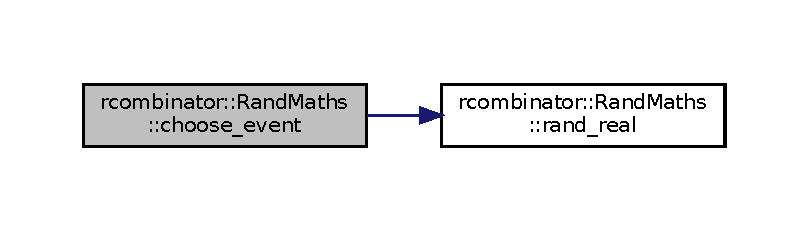
\includegraphics[width=350pt]{classrcombinator_1_1RandMaths_afbc0d35bd9744ecab1983914ac32d68c_cgraph}
\end{center}
\end{figure}
\mbox{\Hypertarget{classrcombinator_1_1RandMaths_aa96396651fba75ffb972b5fa1c2994c7}\label{classrcombinator_1_1RandMaths_aa96396651fba75ffb972b5fa1c2994c7}} 
\index{rcombinator\+::\+Rand\+Maths@{rcombinator\+::\+Rand\+Maths}!initialize\+Rand\+Maths@{initialize\+Rand\+Maths}}
\index{initialize\+Rand\+Maths@{initialize\+Rand\+Maths}!rcombinator\+::\+Rand\+Maths@{rcombinator\+::\+Rand\+Maths}}
\subsubsection{\texorpdfstring{initialize\+Rand\+Maths()}{initializeRandMaths()}}
{\footnotesize\ttfamily \mbox{\hyperlink{classrcombinator_1_1RandMaths}{Rand\+Maths}} \& Rand\+Maths\+::initialize\+Rand\+Maths (\begin{DoxyParamCaption}\item[{long}]{seed = {\ttfamily 0} }\end{DoxyParamCaption})\hspace{0.3cm}{\ttfamily [static]}}



Returns an instance of a \mbox{\hyperlink{classrcombinator_1_1RandMaths}{Rand\+Maths}} class, after seeding it. 

Can be done only once as we want to share the random number generation among all other classes, and seed only once for controlling the numbers that are generated. If the seed is set to the special value 0 during construction, the seed is randomly chosen using system time. \mbox{\Hypertarget{classrcombinator_1_1RandMaths_ae417da209eb8a9d1b2217e7a5397926c}\label{classrcombinator_1_1RandMaths_ae417da209eb8a9d1b2217e7a5397926c}} 
\index{rcombinator\+::\+Rand\+Maths@{rcombinator\+::\+Rand\+Maths}!rand\+\_\+int@{rand\+\_\+int}}
\index{rand\+\_\+int@{rand\+\_\+int}!rcombinator\+::\+Rand\+Maths@{rcombinator\+::\+Rand\+Maths}}
\subsubsection{\texorpdfstring{rand\+\_\+int()}{rand\_int()}}
{\footnotesize\ttfamily int Rand\+Maths\+::rand\+\_\+int (\begin{DoxyParamCaption}\item[{int}]{low,  }\item[{int}]{high }\end{DoxyParamCaption})}



Generates a random integer within a range. 

The bounds are \mbox{[}inclusive\+\_\+low, exclusive\+\_\+high). Here is the caller graph for this function\+:
\nopagebreak
\begin{figure}[H]
\begin{center}
\leavevmode
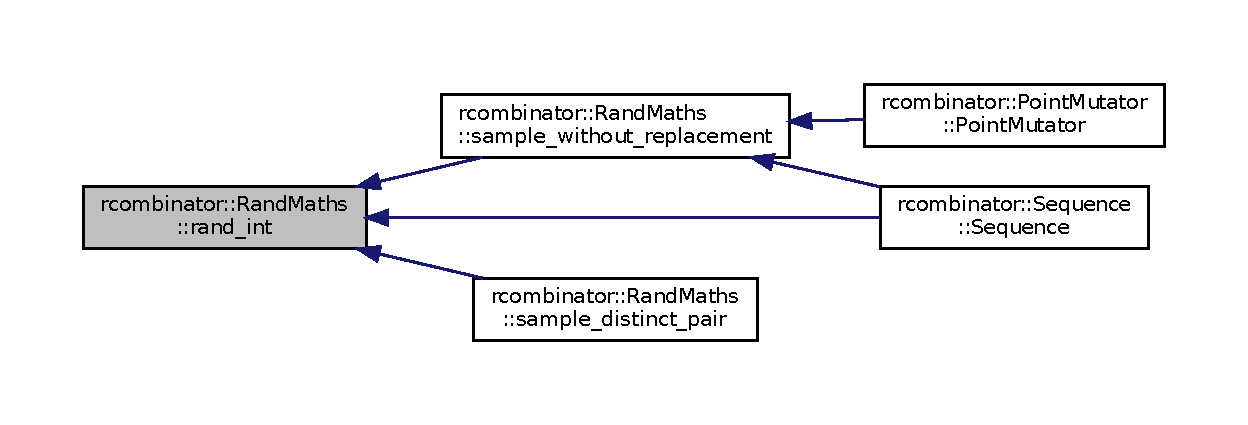
\includegraphics[width=350pt]{classrcombinator_1_1RandMaths_ae417da209eb8a9d1b2217e7a5397926c_icgraph}
\end{center}
\end{figure}
\mbox{\Hypertarget{classrcombinator_1_1RandMaths_a1fec117f0ebd5a7834fdcf649a23edd7}\label{classrcombinator_1_1RandMaths_a1fec117f0ebd5a7834fdcf649a23edd7}} 
\index{rcombinator\+::\+Rand\+Maths@{rcombinator\+::\+Rand\+Maths}!rand\+\_\+poisson@{rand\+\_\+poisson}}
\index{rand\+\_\+poisson@{rand\+\_\+poisson}!rcombinator\+::\+Rand\+Maths@{rcombinator\+::\+Rand\+Maths}}
\subsubsection{\texorpdfstring{rand\+\_\+poisson()}{rand\_poisson()}}
{\footnotesize\ttfamily long Rand\+Maths\+::rand\+\_\+poisson (\begin{DoxyParamCaption}\item[{double}]{mean }\end{DoxyParamCaption})}



Chooses a number sampled from a Poisson distribution. 

Takes the mean as a parameter. \mbox{\Hypertarget{classrcombinator_1_1RandMaths_aa6441baa59bff50f588c0c54e3c54140}\label{classrcombinator_1_1RandMaths_aa6441baa59bff50f588c0c54e3c54140}} 
\index{rcombinator\+::\+Rand\+Maths@{rcombinator\+::\+Rand\+Maths}!rand\+\_\+real@{rand\+\_\+real}}
\index{rand\+\_\+real@{rand\+\_\+real}!rcombinator\+::\+Rand\+Maths@{rcombinator\+::\+Rand\+Maths}}
\subsubsection{\texorpdfstring{rand\+\_\+real()}{rand\_real()}}
{\footnotesize\ttfamily double Rand\+Maths\+::rand\+\_\+real (\begin{DoxyParamCaption}\item[{double}]{low = {\ttfamily 0.0},  }\item[{double}]{high = {\ttfamily 1.0} }\end{DoxyParamCaption})}



Generates a random real number within a range. 

The bounds are \mbox{[}inclusive\+\_\+low, exclusive high). Here is the caller graph for this function\+:
\nopagebreak
\begin{figure}[H]
\begin{center}
\leavevmode
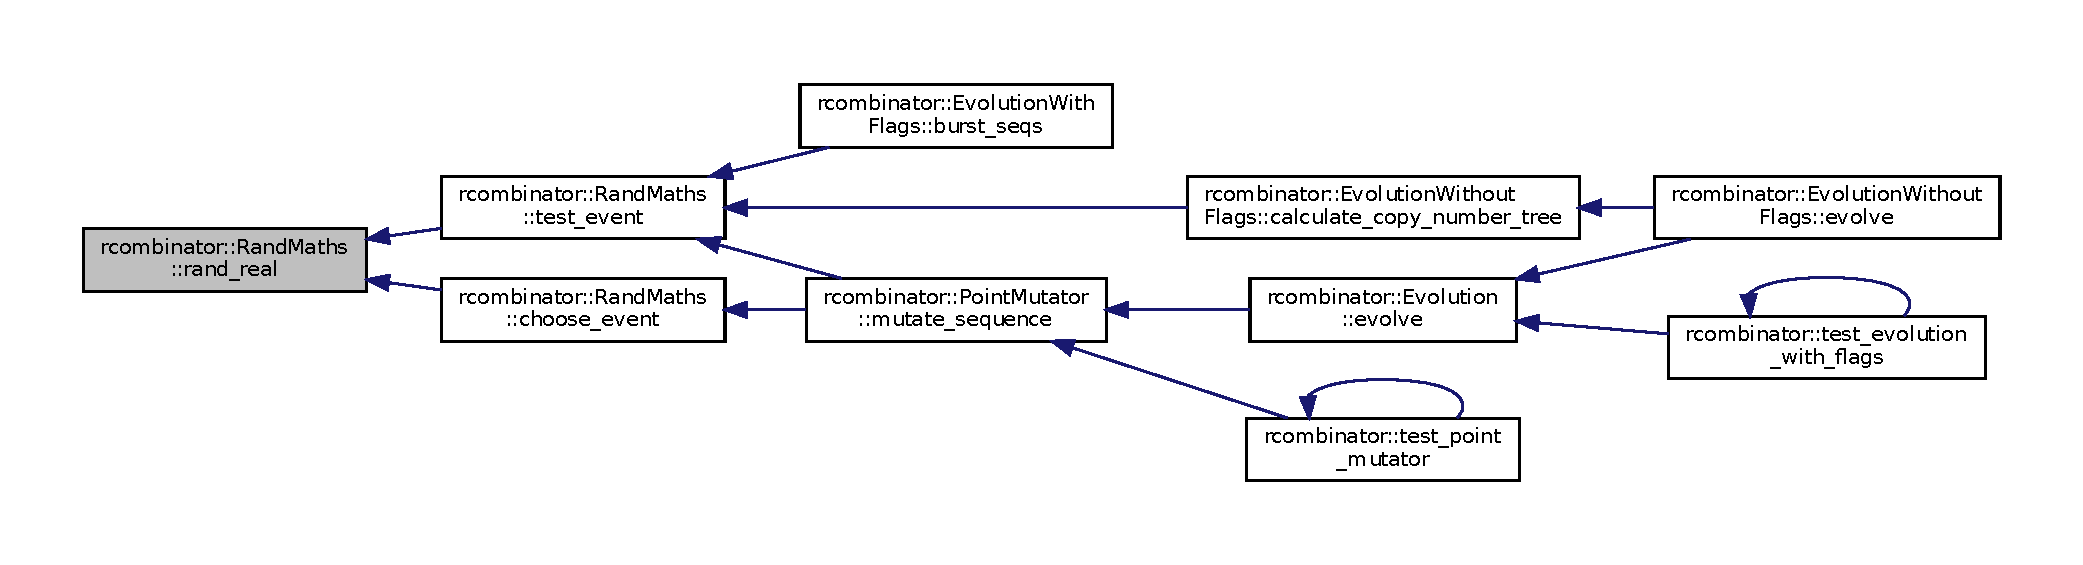
\includegraphics[width=350pt]{classrcombinator_1_1RandMaths_aa6441baa59bff50f588c0c54e3c54140_icgraph}
\end{center}
\end{figure}
\mbox{\Hypertarget{classrcombinator_1_1RandMaths_aaa759efa3059b6793100cb6b6442f26d}\label{classrcombinator_1_1RandMaths_aaa759efa3059b6793100cb6b6442f26d}} 
\index{rcombinator\+::\+Rand\+Maths@{rcombinator\+::\+Rand\+Maths}!sample\+\_\+distinct\+\_\+pair@{sample\+\_\+distinct\+\_\+pair}}
\index{sample\+\_\+distinct\+\_\+pair@{sample\+\_\+distinct\+\_\+pair}!rcombinator\+::\+Rand\+Maths@{rcombinator\+::\+Rand\+Maths}}
\subsubsection{\texorpdfstring{sample\+\_\+distinct\+\_\+pair()}{sample\_distinct\_pair()}}
{\footnotesize\ttfamily std\+::pair$<$ int, int $>$ Rand\+Maths\+::sample\+\_\+distinct\+\_\+pair (\begin{DoxyParamCaption}\item[{int}]{low,  }\item[{int}]{high }\end{DoxyParamCaption})}



Samples a non-\/diagonal pair (2 distinct values) within a range. 

The bounds for each value are \mbox{[}inclusive\+\_\+low, exclusive high). Here is the call graph for this function\+:
\nopagebreak
\begin{figure}[H]
\begin{center}
\leavevmode
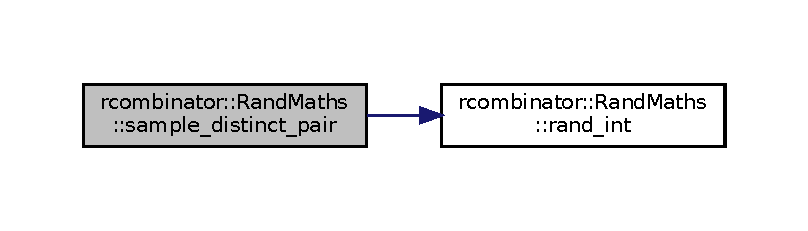
\includegraphics[width=350pt]{classrcombinator_1_1RandMaths_aaa759efa3059b6793100cb6b6442f26d_cgraph}
\end{center}
\end{figure}
\mbox{\Hypertarget{classrcombinator_1_1RandMaths_a2c31949c9ac03952cb0006e6a88e3d85}\label{classrcombinator_1_1RandMaths_a2c31949c9ac03952cb0006e6a88e3d85}} 
\index{rcombinator\+::\+Rand\+Maths@{rcombinator\+::\+Rand\+Maths}!sample\+\_\+without\+\_\+replacement@{sample\+\_\+without\+\_\+replacement}}
\index{sample\+\_\+without\+\_\+replacement@{sample\+\_\+without\+\_\+replacement}!rcombinator\+::\+Rand\+Maths@{rcombinator\+::\+Rand\+Maths}}
\subsubsection{\texorpdfstring{sample\+\_\+without\+\_\+replacement()}{sample\_without\_replacement()}}
{\footnotesize\ttfamily std\+::set$<$ int $>$ Rand\+Maths\+::sample\+\_\+without\+\_\+replacement (\begin{DoxyParamCaption}\item[{int}]{low,  }\item[{int}]{high,  }\item[{int}]{m }\end{DoxyParamCaption})}



Samples {\itshape m} integers within a range, without replacement. 

The bounds are \mbox{[}inclusive\+\_\+low, exclusive high). The integers are returned in ascending order. Here is the call graph for this function\+:
\nopagebreak
\begin{figure}[H]
\begin{center}
\leavevmode
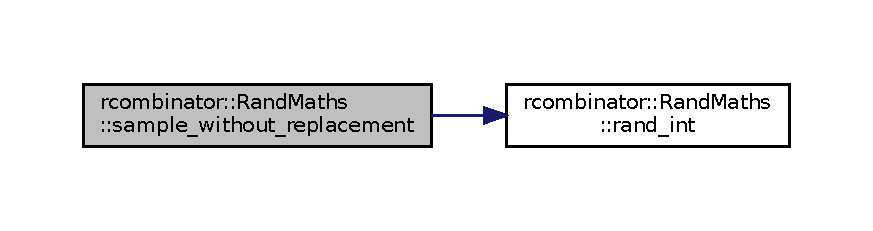
\includegraphics[width=350pt]{classrcombinator_1_1RandMaths_a2c31949c9ac03952cb0006e6a88e3d85_cgraph}
\end{center}
\end{figure}
\mbox{\Hypertarget{classrcombinator_1_1RandMaths_a183686140a9da18ad40c7e048ee8914e}\label{classrcombinator_1_1RandMaths_a183686140a9da18ad40c7e048ee8914e}} 
\index{rcombinator\+::\+Rand\+Maths@{rcombinator\+::\+Rand\+Maths}!test\+\_\+event@{test\+\_\+event}}
\index{test\+\_\+event@{test\+\_\+event}!rcombinator\+::\+Rand\+Maths@{rcombinator\+::\+Rand\+Maths}}
\subsubsection{\texorpdfstring{test\+\_\+event()}{test\_event()}}
{\footnotesize\ttfamily bool Rand\+Maths\+::test\+\_\+event (\begin{DoxyParamCaption}\item[{double}]{event\+\_\+probability }\end{DoxyParamCaption})\hspace{0.3cm}{\ttfamily [inline]}}



Tests whether or not an event happened. 

Takes the probability of an event as paramter, and then compares it to a random value in \mbox{[}0, 1). Here is the call graph for this function\+:
\nopagebreak
\begin{figure}[H]
\begin{center}
\leavevmode
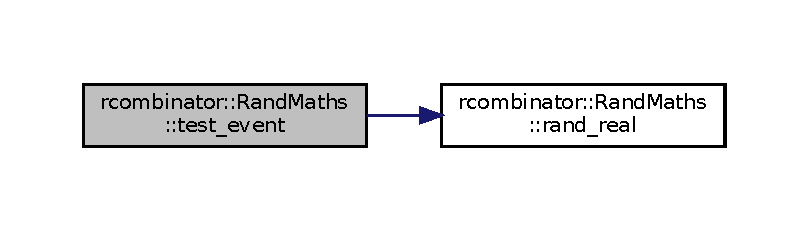
\includegraphics[width=350pt]{classrcombinator_1_1RandMaths_a183686140a9da18ad40c7e048ee8914e_cgraph}
\end{center}
\end{figure}


The documentation for this class was generated from the following files\+:\begin{DoxyCompactItemize}
\item 
src/\mbox{\hyperlink{rand__maths_8h}{rand\+\_\+maths.\+h}}\item 
src/rand\+\_\+maths.\+cpp\end{DoxyCompactItemize}

\hypertarget{structrcombinator_1_1SummaryStats}{}\section{rcombinator\+:\+:Summary\+Stats$<$ T, T\+\_\+cont $>$ Struct Template Reference}
\label{structrcombinator_1_1SummaryStats}\index{rcombinator\+::\+Summary\+Stats$<$ T, T\+\_\+cont $>$@{rcombinator\+::\+Summary\+Stats$<$ T, T\+\_\+cont $>$}}


Plain-\/\+Old-\/\+Data struct to store summary statistics for a list of values.  




{\ttfamily \#include $<$utilities.\+h$>$}

\subsection*{Public Attributes}
\begin{DoxyCompactItemize}
\item 
\mbox{\Hypertarget{structrcombinator_1_1SummaryStats_a19e17a4824f604754cef6b255767e3dc}\label{structrcombinator_1_1SummaryStats_a19e17a4824f604754cef6b255767e3dc}} 
T \mbox{\hyperlink{structrcombinator_1_1SummaryStats_a19e17a4824f604754cef6b255767e3dc}{min}}
\begin{DoxyCompactList}\small\item\em Minimum. \end{DoxyCompactList}\item 
\mbox{\Hypertarget{structrcombinator_1_1SummaryStats_ab44cf45dbe4be027feb8a0d2753ec9d4}\label{structrcombinator_1_1SummaryStats_ab44cf45dbe4be027feb8a0d2753ec9d4}} 
T\+\_\+cont \mbox{\hyperlink{structrcombinator_1_1SummaryStats_ab44cf45dbe4be027feb8a0d2753ec9d4}{q25}}
\begin{DoxyCompactList}\small\item\em First quartile, 25th percentile. \end{DoxyCompactList}\item 
\mbox{\Hypertarget{structrcombinator_1_1SummaryStats_a2fcd7e66d2532d9dec8cb064a020946b}\label{structrcombinator_1_1SummaryStats_a2fcd7e66d2532d9dec8cb064a020946b}} 
T\+\_\+cont \mbox{\hyperlink{structrcombinator_1_1SummaryStats_a2fcd7e66d2532d9dec8cb064a020946b}{median}}
\begin{DoxyCompactList}\small\item\em Median. \end{DoxyCompactList}\item 
\mbox{\Hypertarget{structrcombinator_1_1SummaryStats_a69e4ec6b6049715d315dc6973da873be}\label{structrcombinator_1_1SummaryStats_a69e4ec6b6049715d315dc6973da873be}} 
T\+\_\+cont \mbox{\hyperlink{structrcombinator_1_1SummaryStats_a69e4ec6b6049715d315dc6973da873be}{q75}}
\begin{DoxyCompactList}\small\item\em Third quartile, 75th percentile. \end{DoxyCompactList}\item 
\mbox{\Hypertarget{structrcombinator_1_1SummaryStats_ac2d4ef64bf7cc7a7b9dd74d733daa144}\label{structrcombinator_1_1SummaryStats_ac2d4ef64bf7cc7a7b9dd74d733daa144}} 
T \mbox{\hyperlink{structrcombinator_1_1SummaryStats_ac2d4ef64bf7cc7a7b9dd74d733daa144}{max}}
\begin{DoxyCompactList}\small\item\em Maximum. \end{DoxyCompactList}\item 
\mbox{\Hypertarget{structrcombinator_1_1SummaryStats_a0352cb2fb67bd9653519058608507c45}\label{structrcombinator_1_1SummaryStats_a0352cb2fb67bd9653519058608507c45}} 
T\+\_\+cont \mbox{\hyperlink{structrcombinator_1_1SummaryStats_a0352cb2fb67bd9653519058608507c45}{mean}}
\begin{DoxyCompactList}\small\item\em Arithmetic mean. \end{DoxyCompactList}\end{DoxyCompactItemize}


\subsection{Detailed Description}
\subsubsection*{template$<$typename T, typename T\+\_\+cont$>$\newline
struct rcombinator\+::\+Summary\+Stats$<$ T, T\+\_\+cont $>$}

Plain-\/\+Old-\/\+Data struct to store summary statistics for a list of values. 

Is templated on T and T\+\_\+cont, where T is a numeric type, and T\+\_\+cont is a numeric type that can store fractional parts. Stores the quartiles and the mean for a list of values. 

The documentation for this struct was generated from the following file\+:\begin{DoxyCompactItemize}
\item 
src/\mbox{\hyperlink{utilities_8h}{utilities.\+h}}\end{DoxyCompactItemize}

\chapter{File Documentation}
\hypertarget{exception_8h}{}\doxysection{src/exception.h File Reference}
\label{exception_8h}\index{src/exception.h@{src/exception.h}}
{\ttfamily \#include $<$string$>$}\newline
Include dependency graph for exception.\+h\+:
\nopagebreak
\begin{figure}[H]
\begin{center}
\leavevmode
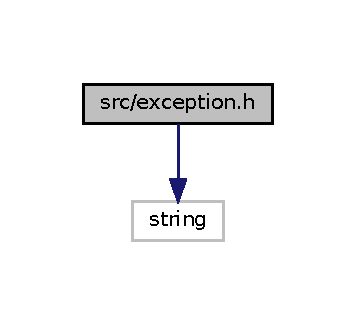
\includegraphics[width=171pt]{exception_8h__incl}
\end{center}
\end{figure}
This graph shows which files directly or indirectly include this file\+:
\nopagebreak
\begin{figure}[H]
\begin{center}
\leavevmode
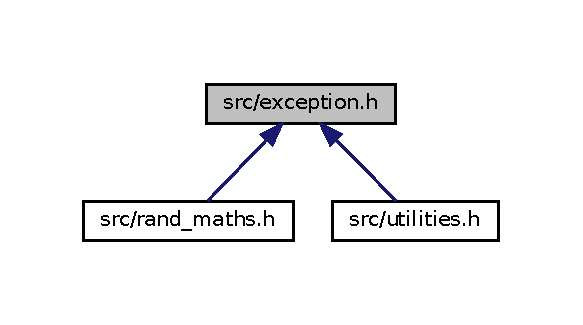
\includegraphics[width=350pt]{exception_8h__dep__incl}
\end{center}
\end{figure}
\doxysubsection*{Classes}
\begin{DoxyCompactItemize}
\item 
class \mbox{\hyperlink{classretrocombinator_1_1Exception}{retrocombinator\+::\+Exception}}
\begin{DoxyCompactList}\small\item\em Basic class to represent exceptions. \end{DoxyCompactList}\end{DoxyCompactItemize}
\doxysubsection*{Namespaces}
\begin{DoxyCompactItemize}
\item 
 \mbox{\hyperlink{namespaceretrocombinator}{retrocombinator}}
\end{DoxyCompactItemize}

\hypertarget{rand__maths_8h}{}\section{src/rand\+\_\+maths.h File Reference}
\label{rand__maths_8h}\index{src/rand\+\_\+maths.\+h@{src/rand\+\_\+maths.\+h}}


Declaration of the global random number generator.  


{\ttfamily \#include \char`\"{}constants.\+h\char`\"{}}\newline
{\ttfamily \#include $<$chrono$>$}\newline
{\ttfamily \#include $<$random$>$}\newline
{\ttfamily \#include $<$set$>$}\newline
Include dependency graph for rand\+\_\+maths.\+h\+:\nopagebreak
\begin{figure}[H]
\begin{center}
\leavevmode
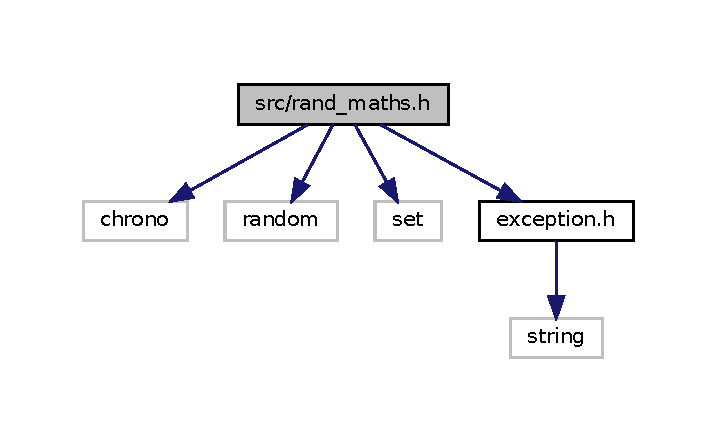
\includegraphics[width=344pt]{rand__maths_8h__incl}
\end{center}
\end{figure}
This graph shows which files directly or indirectly include this file\+:\nopagebreak
\begin{figure}[H]
\begin{center}
\leavevmode
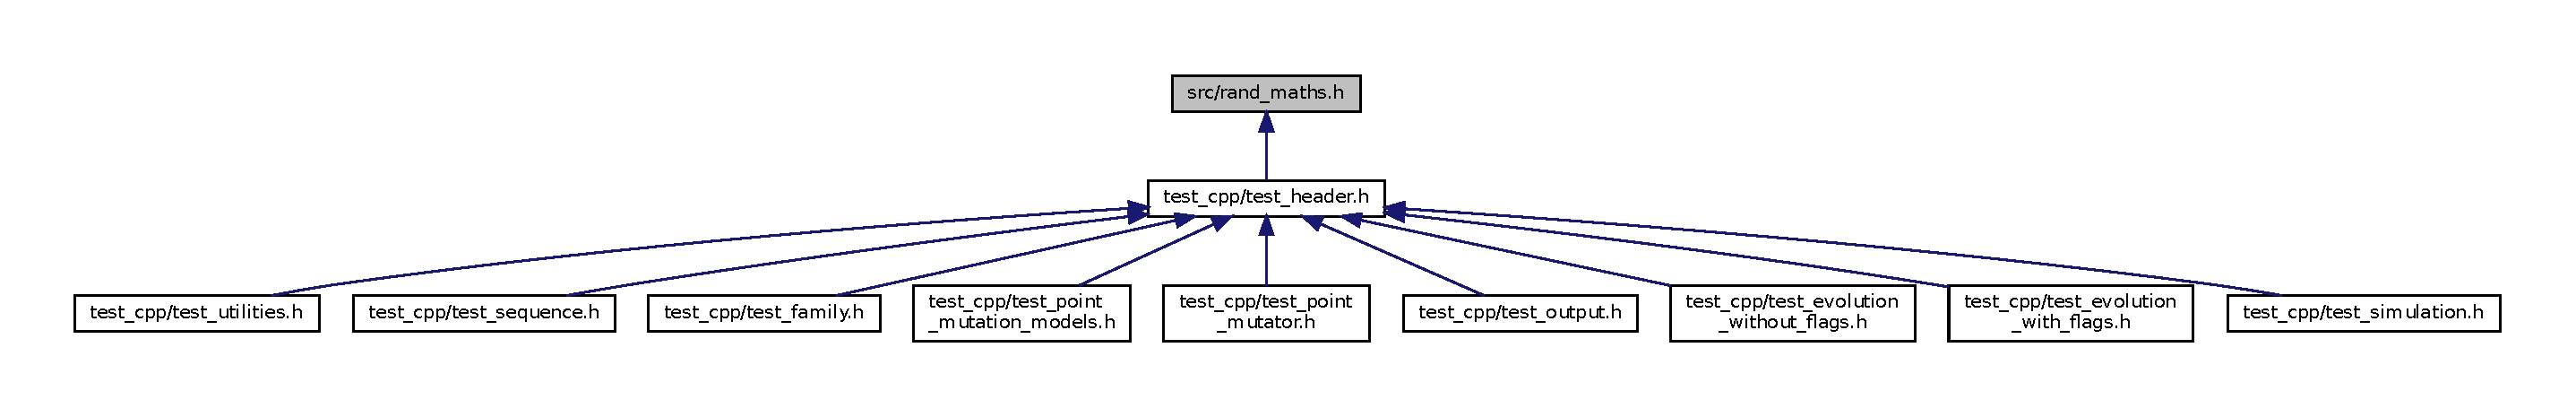
\includegraphics[width=350pt]{rand__maths_8h__dep__incl}
\end{center}
\end{figure}
\subsection*{Classes}
\begin{DoxyCompactItemize}
\item 
class \hyperlink{classretrocombinator_1_1RandMaths}{retrocombinator\+::\+Rand\+Maths}
\begin{DoxyCompactList}\small\item\em For all maths helper functions that use random number generation. \end{DoxyCompactList}\end{DoxyCompactItemize}


\subsection{Detailed Description}
Declaration of the global random number generator. 

Used for basic methods in statistics and probability. R\+NG is the global instance name. 
\hypertarget{utilities_8h}{}\section{src/utilities.h File Reference}
\label{utilities_8h}\index{src/utilities.\+h@{src/utilities.\+h}}


Definitions of basic helper functions.  


{\ttfamily \#include $<$algorithm$>$}\newline
{\ttfamily \#include $<$cmath$>$}\newline
{\ttfamily \#include $<$vector$>$}\newline
{\ttfamily \#include \char`\"{}exception.\+h\char`\"{}}\newline
Include dependency graph for utilities.\+h\+:\nopagebreak
\begin{figure}[H]
\begin{center}
\leavevmode
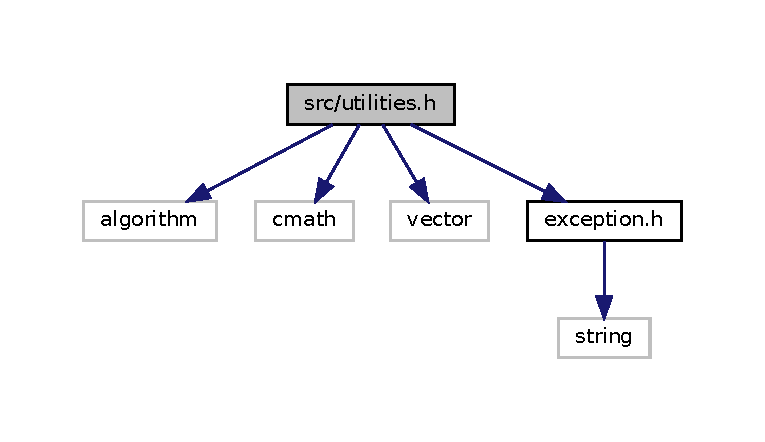
\includegraphics[width=350pt]{utilities_8h__incl}
\end{center}
\end{figure}
\subsection*{Classes}
\begin{DoxyCompactItemize}
\item 
struct \mbox{\hyperlink{structrcombinator_1_1Utils_1_1SummaryStats}{rcombinator\+::\+Utils\+::\+Summary\+Stats$<$ T, T\+\_\+cont $>$}}
\begin{DoxyCompactList}\small\item\em Plain-\/\+Old-\/\+Data struct to store summary statistics for a list of values. \end{DoxyCompactList}\end{DoxyCompactItemize}
\subsection*{Namespaces}
\begin{DoxyCompactItemize}
\item 
 \mbox{\hyperlink{namespacercombinator_1_1Utils}{rcombinator\+::\+Utils}}
\begin{DoxyCompactList}\small\item\em To store some useful functions in a namespace and prevent conflicts. \end{DoxyCompactList}\end{DoxyCompactItemize}
\subsection*{Functions}
\begin{DoxyCompactItemize}
\item 
bool \mbox{\hyperlink{namespacercombinator_1_1Utils_aa38fa31292dbf3a06522dc76b20e2572}{rcombinator\+::\+Utils\+::is\+\_\+in\+\_\+range}} (long test, long lb, long ub)
\begin{DoxyCompactList}\small\item\em Checks whether a number lies within a range. \end{DoxyCompactList}\end{DoxyCompactItemize}


\subsection{Detailed Description}
Definitions of basic helper functions. 

A collection of short, useful functions and data structures 
%--- End generated contents ---

% Index
\backmatter
\newpage
\phantomsection
\clearemptydoublepage
\addcontentsline{toc}{chapter}{Index}
\printindex

\end{document}
